\documentclass{article}

\usepackage{graphicx}
\graphicspath{ {./images/} }

\title{Ch. 22 HW \#3 -- Solutions}
\author{Principles of Microeconomics}
\date{\today}

\begin{document}

\maketitle

\subsection*{Quick Quiz}

\begin{enumerate}
\setcounter{enumi}{4}

\item (b) -- Consumers' chosen bundle is their optimal bundle. At an optimal bundle, the marginal rate of substitution equals the negative slope of the budget constraint. Here, the negative slope of the budget constraint is \\ $\frac{P_{shirt}}{P_{hat}} = 2$.

\item (d) -- An increase in the price of peanut butter decreases Maggie's purchasing power (the amount of stuff she can buy), so she effectively becomes poorer. Demand for normal goods goes down when people become poorer, so Maggie buys less of both goods.

\item (c) -- When the price of wine rises, wine becomes relatively more expensive, and bread becomes relatively cheaper. Ned will substitute away from the more expensive good and towards the cheaper good, so he'll buy less wine and more bread.

\end{enumerate}

\subsection*{Problems \& Applications}

\begin{enumerate}

\item

	\begin{enumerate}
	
	\item \phantom{x}
	
		\begin{center}
		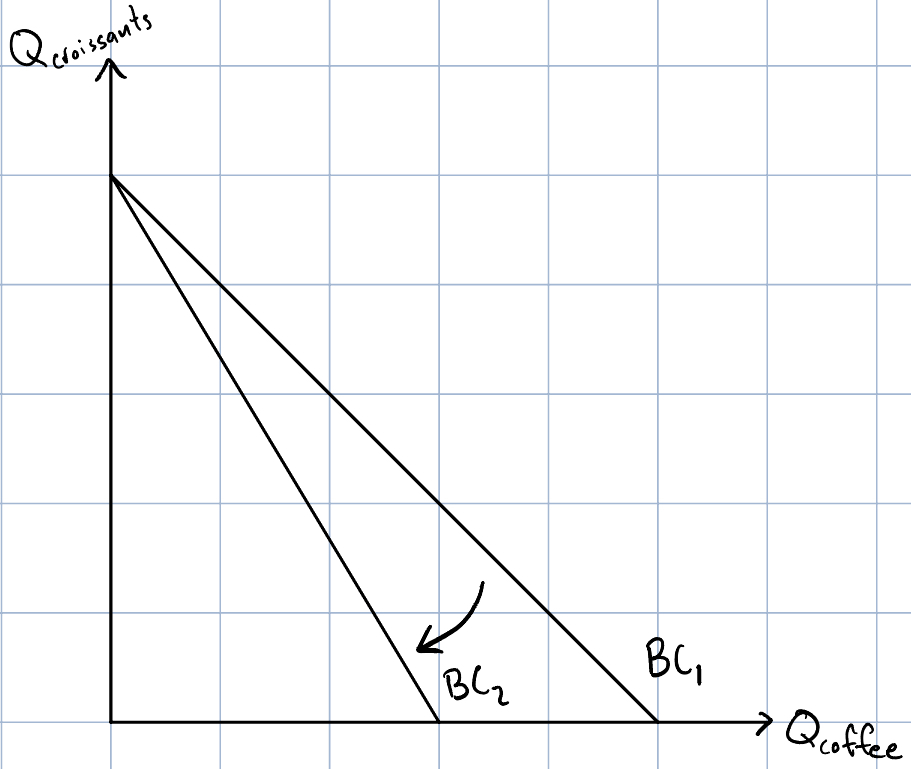
\includegraphics[width = 0.5\textwidth]{paa1a}
		\end{center}
		
	\item An increase in the coffee price makes Maya effectively poorer. Since croissants are a normal good, the income effect will be negative because people demand less of a normal good when they become poorer. The increase in the coffee price also makes croissants relatively cheaper. Maya will substitute towards croissant consumption, so the substitution effect is positive. If the substitution effect outweighs the income effect, she will end up consuming more croissants. 
	
		\begin{center}
		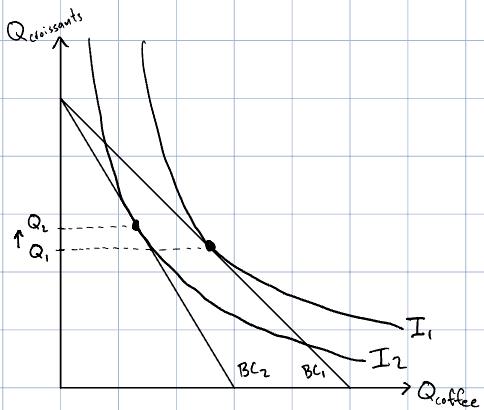
\includegraphics[width = 0.5\textwidth]{paa1b}
		\end{center}
		
	\item For the same reasons as in (b), the income effect is negative, but the substitution effect is positive. If the income effect outweighs the substitution effect, she will consume fewer croissants.
	
		\begin{center}
		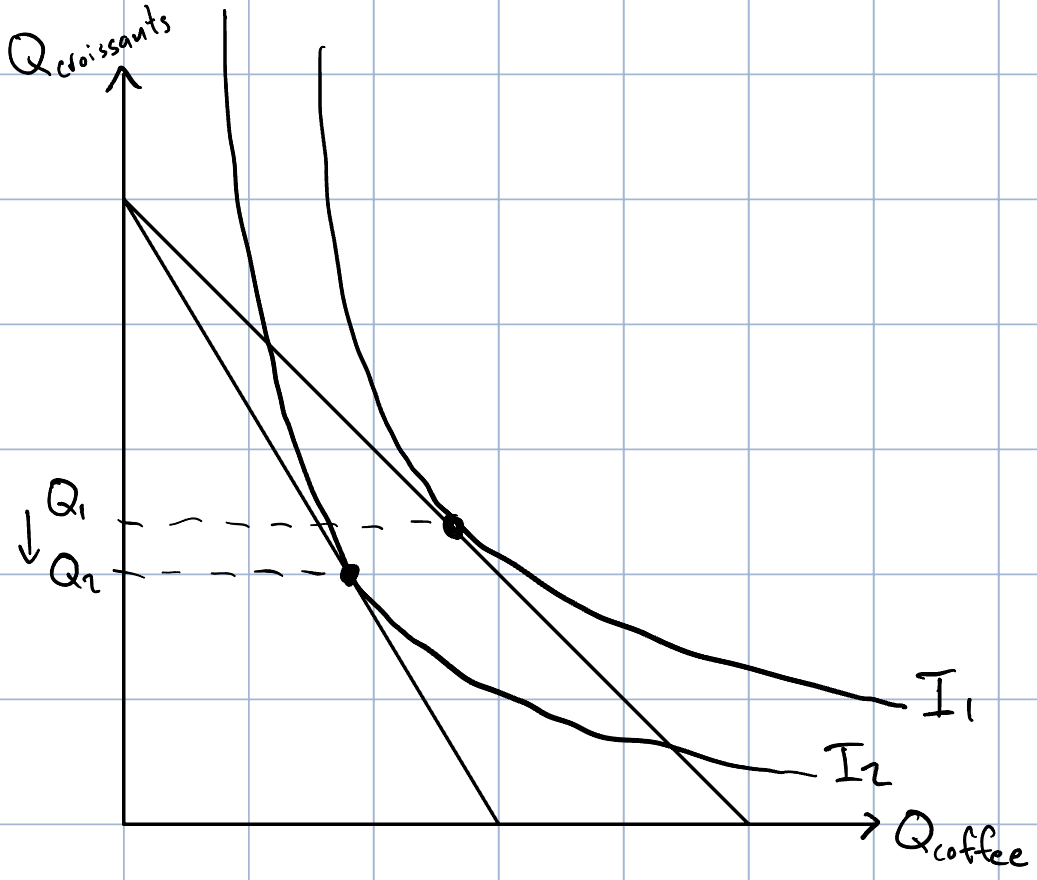
\includegraphics[width = 0.5\textwidth]{paa1c}
		\end{center}
	
	\end{enumerate}
	
\item

	\begin{enumerate}
	
	\item Coke and Pepsi are substitutes because one is usually consumed in lieu of the other. Skis and ski bindings are complements because they are usually consumed together.
	
	\item Indifference curves are straighter for substitutes, so I expect the indifference curves to be fairly straight for Coke and Pepsi. Indifference curves are more curved for complements, so I expect the indifference curves for skis and ski bindings to be very bowed.
	
	\item The consumer will respond more to a change in the relative price of Coke and Pepsi. Since Coke and Pepsi are close substitutes, a change in their relative price will cause the consumer to substitute significantly towards the cheaper option. In the case of skis and ski bindings, a change in their relative price won't affect consumption as much. Since the consumer typically buys them together, their combined price matters more than their relative prices.  
	
	\end{enumerate}
	
\item

	\begin{enumerate}
	
	\item Since you're just as happy as you were before the price changes, that means you're indifferent between your original optimal bundle and your new optimal bundle after the price changes. That means the two bundles must be on the same indifference curve.
	
		\begin{center}
		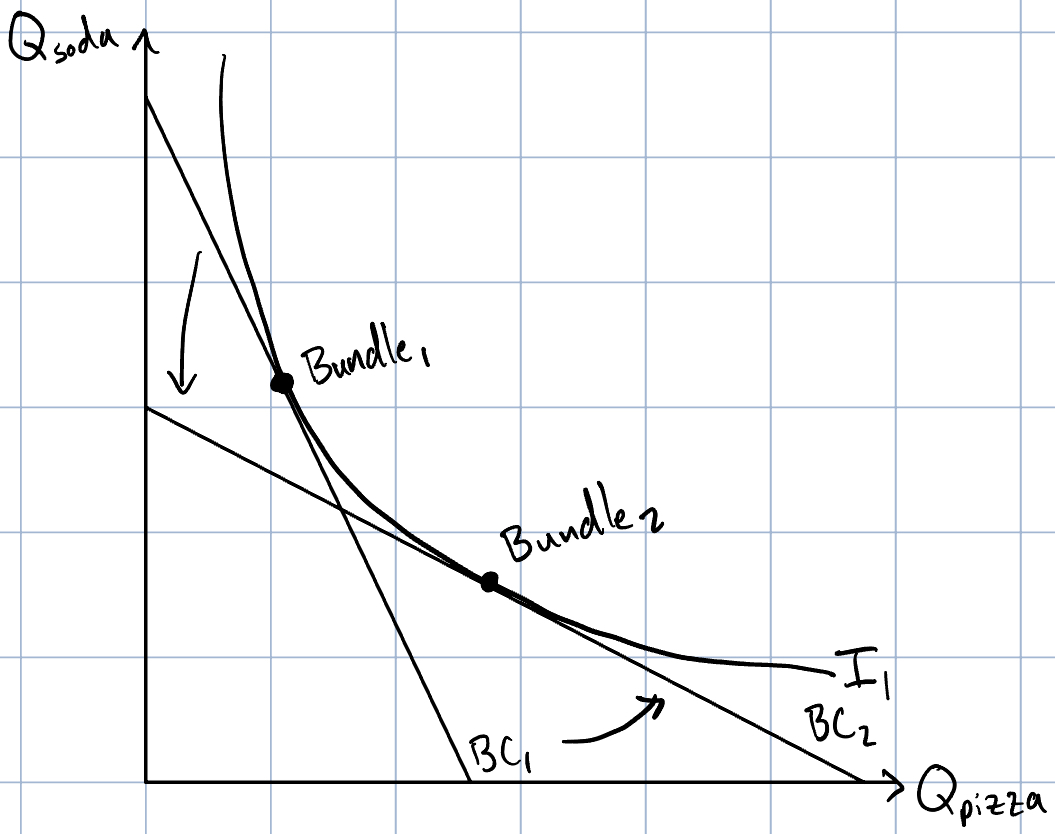
\includegraphics[width = 0.5\textwidth]{paa3a}
		\end{center}
	
	\item Your consumption of soda goes down, and your consumption of pizza goes up. That response stems entirely from the substitution effect and not at all from the income effect. Since you stay on the same indifference curve after the price change, you aren't effectively poorer or richer. You're just as well off as you were before. That means there is no income effect. There is a substitution effect because the relative prices of the goods changed. 
	
		\begin{center}
		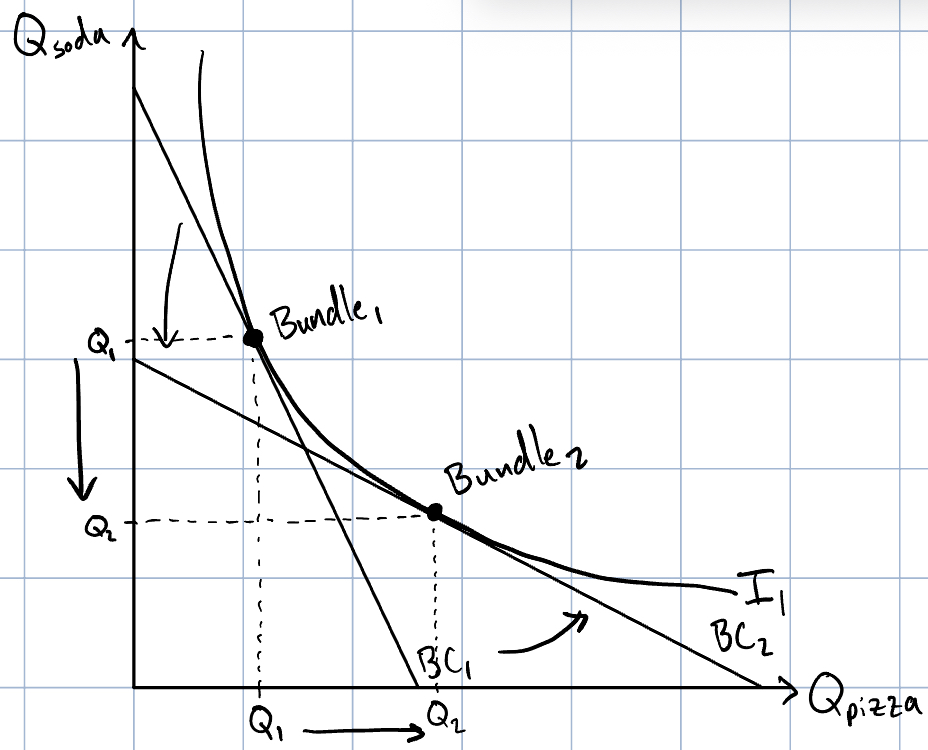
\includegraphics[width=0.5\textwidth]{paa3b}
		\end{center}
	
	\item You cannot. It's outside of $BC_2$, so it is beyond your budget.
	
	\end{enumerate}

\end{enumerate}

\end{document}